\documentclass[10pt, a4paper]{article}
\usepackage[utf8]{inputenc}
\usepackage{mathtools}
\usepackage{array}
\usepackage[italian]{babel}
\usepackage[pdfusetitle]{hyperref}
\usepackage{cancel}
\usepackage{xcolor}
\usepackage[pdftex]{graphicx}
\usepackage{caption}
\usepackage{titling}
\usepackage{comment}

\title{Il formulario bellino}
\author{Lorenzo Cauli}

\setlength{\footskip}{90pt}
\setlength{\droptitle}{-10em}
\graphicspath{./images/}


\begin{document}
    \maketitle
    \hspace{-35pt}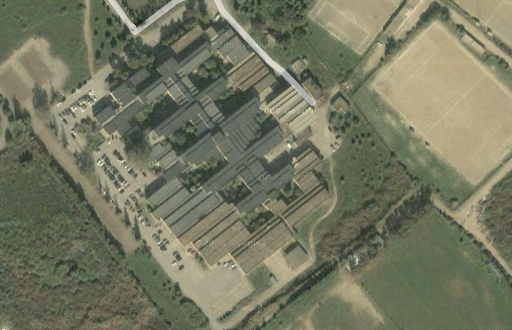
\includegraphics[width=400pt]{images/scano.png}
    \newpage
    \tableofcontents

    \newpage
    \section{Derivate}
    \documentclass[../../main]{subfiles}
\begin{document}
\subsection{Funzioni Razionali}
\begin{center}
    \noindent\makebox[\textwidth]{
        \label{tab:derivate:razionali}
        \begin{tabular}{ |p{5em}|p{5em}|p{5em}|p{7em}|p{5cm}| }
            \hhline{|=|=|=|=|=|}
            Nome & Formula & Derivata & Esempio & Nota \\
            
            \hline
            
            % funzioni costanti
            \begin{align*}
		    \text{Costante}
            \end{align*} &
            \begin{align*}
                y=n 
            \end{align*}  &
            \begin{align*}
                y'=0 
            \end{align*} &
            {
                \begin{align*}
                    y &= 4    \\
                    y' & = 0  
                \end{align*}
            } &
            \begin{center}
                La derivata di qualsiasi funzione costante equivale a 0 
            \end{center} \\ 

            \hline
            
            % razionali intere
            \begin{align*}
		    \text{Intera}
            \end{align*} &
            \begin{align*}
                y=x^n 
            \end{align*} &
            \begin{align*}
                y'=nx^{n-1} 
            \end{align*} &
            {
                \begin{align*}
                    y  & = 5x^2         \\
                    y' & =(2*5)x^{2-1}  \\
                        & =10x          
                \end{align*}
            } &  \\

            \hline
            
            % razionali frazionarie
            \begin{align*}
		    \text{Frazionaria}
            \end{align*} &
            \begin{align*}
                y = \frac{n}{x} 
            \end{align*} &
            \begin{center}
                ---
            \end{center} &
            \begin{center}
                ---
            \end{center} &
            \begin{center}
                Vedere "Rapporto" sezione \nameref{tab:derivate:operazioni} a pagina \pageref{tab:derivate:operazioni} \\
            \end{center}  \\
            \hhline{|=|=|=|=|=|}
        \end{tabular}
    }
\end{center}

\end{document}

    \documentclass[../../main]{subfiles}
\begin{document}
\subsection{Funzioni Irrazionali}
\begin{center}
    \noindent\makebox[\textwidth]{
        \label{tab:derivate:irrazionali}
        \begin{tabular}{ |p{5em}|p{5em}|p{5em}|p{7em}|p{5cm}| }
            \hline
            Nome & Formula & Derivata & Esempio & Nota \\
            
            \hline
            
            % funzioni costanti
            \begin{center}
                Radice quadrata
            \end{center} &
            \begin{align}
                y=\sqrt{x} \nonumber
            \end{align}  &
            \begin{align}
                y'=\frac{1}{ 2\sqrt{x} } \nonumber
            \end{align} &
            {
                \begin{align}
                    y  &= \sqrt{x^4}   \nonumber \\
                        &= x^\frac{4}{2}  \nonumber \\
                    y' &= \frac{\cancel{4}^2}{\cancel{2}_1}x^{\frac{\cancel{4}^2}{\cancel{2}_1}-1} \nonumber \\
                        &= 2x^{2-1} \nonumber \\
                        &= 2x \nonumber 
                \end{align}
            } &
            \begin{center}
                La radice quadrata puo' essere espressa come potenza, quindi si puo' applicare la regola per le funzioni razionali intere.
            \end{center} \\ 

            \hline
            
        \end{tabular}
    }
\end{center}

\end{document}
    \subsection{Funzioni Esponenziali}
\begin{center}
    \noindent\makebox[\textwidth]{
        \label{tab:derivate:esponenziali}
        \begin{tabular}{ |p{5em}|p{5em}|p{5em}|p{7em}|p{5cm}| }
            \hline
            Nome & Formula & Derivata & Esempio & Nota \\
            
            \hline
            
            % funzioni costanti
            \begin{center}
                Funzione esponenziale
            \end{center} &
            \begin{align}
                y=n^x \nonumber
            \end{align}  &
            \begin{align}
                y'=n^xln(n) \nonumber
            \end{align} &
            {
                \begin{align}
                    y  &= \sqrt{x^4}   \nonumber \\
                        &= x^\frac{4}{2}  \nonumber \\
                    y' &= \frac{\cancel{4}^2}{\cancel{2}_1}x^{\frac{\cancel{4}^2}{\cancel{2}_1}-1} \nonumber \\
                        &= 2x^{2-1} \nonumber \\
                        &= 2x \nonumber 
                \end{align}
            } &
            \begin{center}
                La radice quadrata puo' essere espressa come potenza, quindi si puo' applicare la regola per le funzioni razionali intere.
            \end{center} \\ 

            \hline
            
        \end{tabular}
    }
\end{center}
    \documentclass[../../main]{subfiles}
\begin{document}
\subsection{Funzioni Logaritmiche}
\begin{center}
    \noindent\makebox[\textwidth]{
        \label{tab:derivate:logaritmiche}
        \begin{tabular}{ |p{5em}|p{5em}|p{5em}|p{7em}|p{5cm}| }
            \hline
            Nome & Formula & Derivata & Esempio & Nota \\
            
            \hline
            
            % funzioni costanti
            \begin{center}
                Logaritmo
            \end{center} &
            \begin{align}
                y=\log_a{x} \nonumber
            \end{align}  &
            \begin{align}
                y'=\frac{1}{x}\log_a{e} \nonumber
            \end{align} &
            {
                \begin{align}
                    y  &= \sqrt{x^4}   \nonumber \\
                        &= x^\frac{4}{2}  \nonumber \\
                    y' &= \frac{\cancel{4}^2}{\cancel{2}_1}x^{\frac{\cancel{4}^2}{\cancel{2}_1}-1} \nonumber \\
                        &= 2x^{2-1} \nonumber \\
                        &= 2x \nonumber 
                \end{align}
            } &
            {
            \begin{center}
                Se il logaritmo ha come base \emph{e} (quindi si tratta di logaritmo naturale), la formula si puo' contrarre. \\
                Esempio: \\
                \begin{align}
                    y &= \ln{x} \nonumber \\
                    y' &= \frac{1}{x} \nonumber
                \end{align}
            \end{center}
            } \\

            \hline
            
        \end{tabular}
    }
\end{center}

\end{document}
    \subsection{Funzioni Goniometriche}
\begin{center}
    \noindent\makebox[\textwidth]{
        \label{tab:derivate:goniometriche}
        \begin{tabular}{ |p{5em}|p{5em}|p{5em}|p{7em}|p{5cm}| }
            \hline
            Nome & Formula & Derivata & Esempio & Nota \\
            
            \hline
            
            % funzioni costanti
            \begin{center}
                Seno
            \end{center} &
            \begin{align}
                y=\sin{x} \nonumber
            \end{align}  &
            \begin{align}
                y'=\cos{x} \nonumber
            \end{align} &
            {
                \begin{align}
                    y  &= \sqrt{x^4}   \nonumber \\
                        &= x^\frac{4}{2}  \nonumber \\
                    y' &= \frac{\cancel{4}^2}{\cancel{2}_1}x^{\frac{\cancel{4}^2}{\cancel{2}_1}-1} \nonumber \\
                        &= 2x^{2-1} \nonumber \\
                        &= 2x \nonumber 
                \end{align}
            } &
            {
            \begin{center}
            \end{center}
            } \\

            \hline
            
        \end{tabular}
    }
\end{center}
    \documentclass[../../main]{subfiles}
\begin{document}
\subsection{Operazioni tra funzioni}
\begin{center}
        \label{tab:derivate:operazioni}
        \begin{longtable}{ |p{5em} | p{5em} | p{5em} | p{7em} | p{2cm}| }
            \hhline{|=|=|=|=|=|}
            Nome & Formula & Derivata & Esempio & Nota \\
            
            \hline
            
            % somma funzioni
            \begin{center}
                Somma
            \end{center} &
            \begin{align*}
                y= {\color{red}f(x)} + {\color{blue}g(x)} 
            \end{align*}  &
            \begin{align*}
                y'= {\color{red}f'(x)} + {\color{blue}g'(x)} 
            \end{align*} &
            {
                \begin{align*}
                    y  &= {\color{red}x^2} + {\color{blue}4}    \\
                    y' &= {\color{red}2x^{2-1}} + {\color{blue}0}  \\
                        &= 2x  
                \end{align*}
            } &
            \begin{center}
            \end{center} \\ 

            \hline
            
            % differenza funzioni
            \begin{center}
                Differenza
            \end{center} &
            \begin{align*}
                y= {\color{red}f(x)} - {\color{blue}g(x)} 
            \end{align*}  &
            \begin{align*}
                y'= {\color{red}f'(x)} - {\color{blue}g'(x)} 
            \end{align*} &
            {
                \begin{align*}
                    y  &= {\color{red}x^2} - {\color{blue}4}    \\
                    y' &= {\color{red}2x^{2-1}} - {\color{blue}0}  \\
                        &= 2x  
                \end{align*}
            } &
            \begin{center}
            \end{center} \\ 

            \hline
            
            % prodotto funzioni
            \begin{center}
                Prodotto
            \end{center} &
            \begin{align*}
                y= {\color{red}f(x)} * {\color{blue}g(x)} 
            \end{align*}  &
            \begin{align*}
                y'= ({\color{red}f'(x)} * {\color{blue}g(x)} ) + ( {\color{red}f(x)} * {\color{blue}g'(x)}) 
            \end{align*} &
            {
                \begin{align*}
                    y  &= {\color{red}x^2} * {\color{blue}4}    \\
                    y' &= ( {\color{red}2x^{2-1}} * {\color{blue}4} ) + ( {\color{red}x^2} * {\color{blue}0} )  \\
                        &= (2x * 4) + 0  \\
                        &= 8x  
                \end{align*}
            } &
            \begin{center}
            \end{center} \\ 

            \hline
            
            % rapporto funzioni
            \begin{center}
                Rapporto
            \end{center} &
            \begin{align*}
                y= \frac{\color{red}f(x)}{\color{blue}g(x)} 
            \end{align*}  &
            \begin{align*}
                y'= \frac{[{\color{red}f'(x)} * {\color{blue}g(x)} ] - [ {\color{red}f(x)} * {\color{blue}g'(x)}]}{[{\color{blue}g(x)}]^2} 
            \end{align*} &
            {
                \begin{align*}
                    y  &= \frac{\color{red}x^2}{\color{blue}4}    \\
                    y' &= \frac{( {\color{red}2x^{2-1}} * {\color{blue}4} ) - ( {\color{red}x^2} * {\color{blue}0} )}{{\color{blue}4}^2}  \\
                        &= \frac{({\color{red}2x} * {\color{blue}4}) - 0}{16}  \\
                        &= \frac{\cancel{8}^1x}{\cancel{16}_2}   \\
                        &= \frac{x}{2} 
                \end{align*}
            } &
            \begin{center}
            \end{center} \\ 

            \hline
            
            % funzioni composte
            \begin{center}
                Funzioni composte
            \end{center} &
            \begin{align*}
                y= {\color{red}f({\color{blue}g(x)})} 
            \end{align*}  &
            \begin{align*}
                y'= {\color{red}f'({\color{blue}g(x)})} * {\color{blue}g'(x)} 
            \end{align*} &
            {
                \begin{align*}
                    y  &= {\color{red}sin({\color{blue}2x^2})}    \\
                    y' &= {\color{red}cos({\color{blue}2x^2})} * {\color{blue}4x}  
                \end{align*}
            } &
            \begin{center}
            \end{center} \\ 

            \hhline{|=|=|=|=|=|}
            
        \end{longtable}
\end{center}

\end{document}


    \newpage
    \section{Integrali}
    \subsection{AAAA}
    \huge{WIP}

\end{document} 